% Capítulo 3
\chapter{Objetos Float - Figuras, Tabelas, Algoritmos e Código Fonte}\label{cap:float}

Neste capítulo, irei falar sobre objetos do tipo \texttt{float}, que recebem este nome porque ``flutuam'' no documento, e têm seus lugares finais influenciados por sugestões dadas pelos autores, mas que o \LaTeX{} tem a decisão final sobre onde os colocar. Os principais objetos \texttt{float}\index{float} são as figuras, tabelas, algoritmos e listagens de códigos. 

As seções a seguir contêm exemplos do uso desses quatro tipos de objetos \texttt{float}, bem como de alguns pacotes auxiliares que foram incorporados a este modelo de dissertação/tese.

O pacote \texttt{pdflscape}\index{pdflscape} adiciona o suporte \gls{pdf}\index{PDF} ao ambiente \textit{landscape}\index{landscape} (orientação paisagem) do pacote \texttt{lscape}\index{lscape}. Páginas marcadas com o atributo que indica essa orientação serão rotacionadas e mostradas em modo paisagem pelos visualizadores de arquivos \gls{pdf}. O manual desse pacote pode ser acessado em \url{http://mirrors.ctan.org/macros/latex/contrib/pdflscape/pdflscape.pdf} \parencite{pdflscape}.

O pacote \texttt{float}\index{float} melhora a interface para a definição de objetos \texttt{float}, introduzindo os objetos \textit{boxed float}\index{boxed float}, \textit{ruled float}\index{ruled float} e \textit{plaintop float}\index{plaintop float}. O primeiro tipo de objeto cria floats com um retângulo ao redor dos objetos, enquanto que os dois últimos tipos são mais usados para mostrar códigos. Entretanto, o pacote \texttt{minted}\index{minted}, mostrado na Seção \ref{sec:codigo} provê uma visualização muito mais elegante, de modo que sugiro que use o \texttt{minted} para diagramar seus códigos em \LaTeX{}.

O pacote \texttt{float} ainda define a opção \texttt{H} para colocação de \textit{floats}, que força o \LaTeX{} a colocar um objeto \texttt{float} exatamente naquele lugar (deixando assim de ser um objeto \texttt{float}), mesmo que isso implique em deixar uma parte da página anterior em branco, sem texto. Use essa opção com parcimônia, pois ela pode quebrar o seu texto e gerar uma diagramação esquisita. O manual do pacote \texttt{float}\index{float} pode ser acessado em \url{http://mirrors.ctan.org/macros/latex/contrib/float/float.pdf} \parencite{float}.

O pacote \texttt{adjustbox}\index{adjustbox} pode ser usado para ajustar conteúdo dentro de uma caixa ``virtual'', alterando sua escala, orientação e cortar parte do conteúdo. Esse pacote pode ser aplicado a qualquer objeto \texttt{float} ou até a texto. Os textos destacados dentro de caixas e centralizados que aparecem nos Capítulos \ref{cap:modelo}, \ref{cap:diagramacao}  e outros ainda não vistos, foram produzidos usando o pacote \texttt{adjustbox}. Você também pode usar o \texttt{adjustbox} para diminuir o tamanho de uma tabela, por exemplo, quando ela passa um pouco da largura máxima da área reservada para o texto, e uma diminuição da fonte usada gera letras muito pequenas, difíceis de se ver. Nesse caso, um pequeno ajuste do tamanho da tabela pode ser a melhor opção. Você deve usar essa opção com cuidado, pois uma mudança muito grande pode afetar a qualidade da saída.

\section{Figuras}

Como recomendo o uso do processador \hologo{pdfLaTeX}\index{\hologo{pdfLaTeX}}, devo informar que o \hologo{pdfLaTeX} permite carregar imagens nos formatos \gls{pdf}\index{PDF}, \gls{png}\index{PNG} e \gls{jpg}\index{JPG}. Algumas ferramentas, como LyX, fazem a conversão \textit{on-the-fly}, facilitando a tarefa do usuário mas adicionando tempo ao processamento do texto. Eu sugiro que você converta suas imagens para um desses formatos antes de carregá-las, economizando tempo de conversão durante a compilação do código \LaTeX{}.

O pacote \texttt{graphicx}\index{graphicx} se baseia no pacote \texttt{graphics}\index{graphics} para prover uma interface para argumentos opcionais para o comando \texttt{\textbackslash{}includegraphics}\index{includegraphics}. O pacote \texttt{graphicx} faz parte do grupo de pacotes \texttt{latex-graphics}\index{latex-graphics}, que é uma das coleções obrigatórias\footnote{As coleções obrigatórias de \LaTeX{} implicam que toda distribuição \LaTeX{} deve possuí-las.} de \LaTeX{}.

Na Figura \ref{fig:phdcomics}  vemos um exemplo do uso do comando \texttt{\textbackslash{}includegraphics} para a inclusão de uma imagem no objeto \texttt{float figure}. Os comandos utilizados para gerar essa figura podem ser vistos no Código \ref{cod:includegraphics}.

\begin{figure}[ht]
	\centering
	
\includegraphics[width=14cm]{./imagens/capitulo3/phd020808s}
	\caption{Tirinha cômica extraída da página \url{phdcomics.com}.}
	\label{fig:phdcomics}
\end{figure}

\begin{listing}[ht]
	\begin{minted}[linenos=true, baselinestretch=1, autogobble, bgcolor=Cornsilk1]{tex}
		\begin{figure}[ht]
		  \centering
		  
\includegraphics[width=12cm]{./imagens/capitulo3/phd020808s}
		  \caption{Tirinha cômica extraída da página \url{phdcomics.com}.}
		  \label{fig:phdcomics}
		\end{figure}
	\end{minted}
\caption{Exemplo de imagem carregada usando o comando \texttt{\textbackslash{}includegraphics}.}
\label{cod:includegraphics}
\end{listing}

O manual disponível em  \url{http://mirrors.ctan.org/macros/latex/required/graphics/grfguide.pdf} \parencite{graphicsguide} se refere à coleção \texttt{latex-graphics}\index{latex-graphics} e descreve os pacotes \texttt{color}\index{color}, \texttt{graphics}\index{graphics} e \texttt{graphicx}\index{graphicx} enquanto que o manual acessível em \url{http://mirrors.ctan.org/macros/latex/required/graphics/graphics.pdf} \parencite{graphics} descreve o pacote \texttt{graphics}. Sugiro a leitura do primeiro manual, principalmente das opções descritas em sua Seção 4.4, que tratam da formatação das imagens carregadas pelo comando \texttt{\textbackslash{}includegraphics}\index{includegraphics}.

\subsection{Sub-figuras}

O pacote \texttt{subfig}\index{subfig} provê suporte para a manipulação e referenciamento de subfiguras\index{subfiguras} e subtabelas\index{subtabelas}, permitindo que elas possam ser referenciadas e/ou descritas separadamente ou até mesmo listadas separadamente na Lista de Figuras. Um exemplo simples de figura composta por subfiguras e que foi contruída usando o pacote \texttt{subfig} pode ser vista na Figura \ref{fig:subfig}. Os comandos necessários para gerar esta figura podem ser vistos no Código \ref{cod:subfig}.

\begin{figure}[ht]
    \centering
    \subfloat[]{
        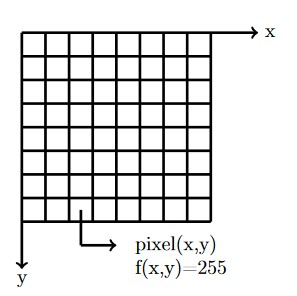
\includegraphics[height=5cm]{imagens/capitulo2/imagemCinza.jpg}}
    \subfloat[]{
        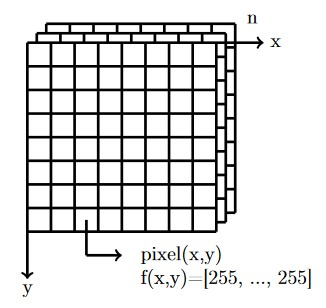
\includegraphics[height=5cm]{imagens/capitulo2/imagemColorida.jpg}}
    \caption{Exemplo de subfiguras usando o pacote \texttt{subfig}. Representação de uma imagem digital. (a) Imagem em escala de cinza. (b) Imagem colorida. Imagem extraída de \parencite{Barbosa2020}.}
    \label{fig:subfig}
\end{figure}

\begin{listing}[ht]
	\begin{minted}[linenos=true, baselinestretch=1, autogobble, bgcolor=Cornsilk1]{tex}
		\begin{figure}[ht]
		  \centering
		  \subfloat[]{
		    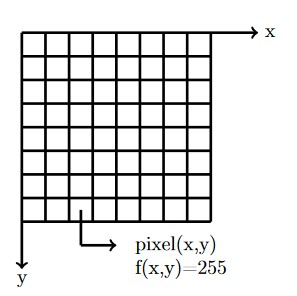
\includegraphics[height=5cm]{imagens/capitulo2/imagemCinza.jpg}}
		  \subfloat[]{
		    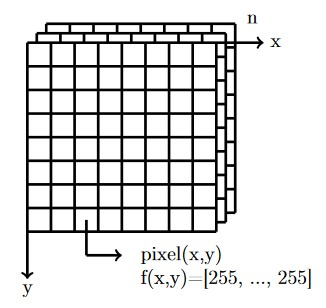
\includegraphics[height=5cm]{imagens/capitulo2/imagemColorida.jpg}}
		  \caption{Exemplo de subfiguras usando o pacote \texttt{subfig}. 
		  Representação de uma imagem digital. (a) Imagem em escala de cinza. 
		  (b) Imagem colorida. Imagem extraída de \parencite{Barbosa2020}.}
		  \label{fig:subfig}
		\end{figure}
	\end{minted}
	\caption{Código usado para organizar subfiguras usando o pacote \texttt{subfig}.}
	\label{cod:subfig}
\end{listing}

Como alternativa, você pode usar o ambiente \texttt{tabular}\index{tabular} para organizar as subfiguras e seus rótulos. A Figura \ref{fig:subfigtabular} foi criada usando este outro modo de organizar subfiguras. O Código \ref{cod:subfigtabular} mostra os comandos usados para gerá-la.

\begin{figure}[H]
	\begin{center}
		\begin{tabular}{cc}
			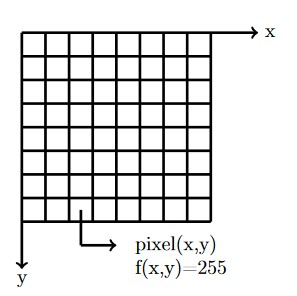
\includegraphics[height=5cm]{imagens/capitulo2/imagemCinza.jpg} & 
			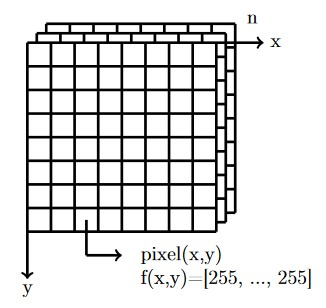
\includegraphics[height=5cm]{imagens/capitulo2/imagemColorida.jpg} \\
			(a) & (b) 
		\end{tabular}
	\end{center}
	\caption{Exemplo de subfiguras\index{subfiguras} usando o ambiente \texttt{tabular}. Representação de uma imagem digital. (a) Imagem em escala de cinza. (b) Imagem colorida. Imagem extraída de \parencite{Barbosa2020}.}
	\label{fig:subfigtabular}
\end{figure}

\begin{listing}[ht]
	\begin{minted}[linenos=true, baselinestretch=1, autogobble, bgcolor=Cornsilk1]{tex}
		\begin{figure}[ht]
		  \begin{center}
		    \begin{tabular}{cc}
		      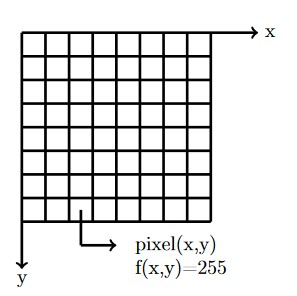
\includegraphics[height=5cm]{imagens/capitulo2/imagemCinza.jpg} & 
		      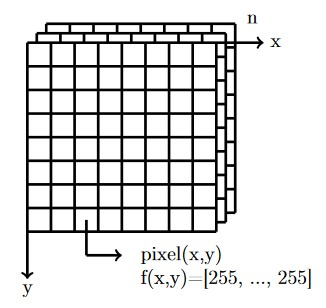
\includegraphics[height=5cm]{imagens/capitulo2/imagemColorida.jpg} 
		      \\
		      (a) & (b) 
		    \end{tabular}
		  \end{center}
		  \caption{Exemplo de subfiguras usando o ambiente \texttt{tabular}. 
		  Representação de uma imagem digital. (a) Imagem em escala de cinza. 
		  (b) Imagem colorida. Imagem extraída de \parencite{Barbosa2020}.}
		  \label{fig:subfigtabular}
		\end{figure}
	\end{minted}
	\caption{Código usado para organizar subfiguras usando o ambiente \texttt{tabular}.}
	\label{cod:subfigtabular}
\end{listing}

Você pode comparar visualmente os resultados das duas opções descritas acima observando as \Cref{fig:subfig,fig:subfigtabular}. Lembre-se que no caso do pacote \texttt{subfig}\index{subfig}, você pode referenciar e listar as subfiguras separadamente. Para maiores detalhes sobre o pacote \texttt{subfig}, consulte seu manual, que está disponível em \url{http://mirrors.ctan.org/macros/latex/contrib/subfig/subfig.pdf} \parencite{subfig}.

\section{Tabelas}

Tabelas são um outro tipo de objeto \texttt{float}\index{float} presente no \LaTeX{}. Existem páginas, capítulos de livros e até livros completos dedicados a criação de tabelas  em \LaTeX{}. Geralmente, se utiliza um ambiente tabular dentro de um objeto \texttt{float} do tipo \texttt{table}\index{table}. Esse ambiente tabular é responsável por informar quantas colunas uma tabela terá, e por sua tabulação, organizando os dados usando delimitadores pré-definidos.

\begin{table}[H]
	\centering
	\resizebox{\textwidth}{!}{%
		\begin{tabular}{|l|l|l|l|l|l|}
			\hline
			Tecido & Distância e Tamanho & Acurácia & Especificidade  & Sensibilidade & Coeficiente de Dice \\ \hline
			\multirow{2}{*}{Granulação} & $9 \times 9$\_E & $0,9252 \pm 0,0796$ & \textbf{$0,8961 \pm 0,1520$} & $0,8478 \pm 0,1942$ & $0,8796 \pm 0,1699$ \\ \cline{2-6}
			& $11 \times 11$\_E\_CSR & \textbf{$0,9292 \pm 0,0755$} & $0,8828 \pm 0,1673$ & \textbf{$0,8983 \pm 0,0914$} & \textbf{$0,9224 \pm 0,0650$} \\ \hline
			\multirow{2}{*}{Necrótico} & $9 \times 9$\_E & \textbf{$0,9595 \pm 0,0518$} & $0,9739 \pm 0,0436$ & $0,8758 \pm 0,8800$ & $0,8215 \pm 0,3155$ \\ \cline{2-6}
			& $11 \times 11$\_E\_CSR & $0,9591 \pm 0,0514$ & \textbf{$0,9741 \pm 0,0379$} & \textbf{$0,8963 \pm 0,0638$} & \textbf{$0,9037 \pm 0,1195$} \\  \hline
			\multirow{2}{*}{Esfacelo} & $9 \times 9$\_E & \textbf{$0,9346 \pm 0,0840$} & \textbf{$1,0000 \pm 0,0000$} & $0,8018 \pm 0,1489$ & \textbf{$0,8825 \pm 0,0983$} \\ \cline{2-6}
			& $11 \times 11$\_E\_CSR & $0,9336 \pm 0,0854$ & \textbf{$1,0000 \pm 0,0000$} & \textbf{$0,8111 \pm 0,1378$} & $0,8707 \pm 0,1089$ \\  \hline
			\multirow{2}{*}{Todos} & $9 \times 9$\_E & $0,9482 \pm 0,0457$ & $0,9784 \pm 0,0309$ & $0,8932 \pm 0,0771$ & $0,9234 \pm 0,0673$ \\ \cline{2-6}
			& $11 \times 11$\_E\_CSR & \textbf{$0,9491 \pm 0,0423$} & \textbf{$0,9788 \pm 0,0298$} & \textbf{$0,8952 \pm 0,0717$} & \textbf{$0,9247 \pm 0,0625$} \\ \hline
		\end{tabular}%
	}
	\caption{Resultados de uma tarefa de agrupamento. Adaptada de \parencite{Marques2018}.}
	\label{tab:resultadosVitor}
\end{table}

A Tabela \ref{tab:resultadosVitor} (adaptada de \parencite{Marques2018}) mostra resultados de uma tarefa de classificação. Neste exemplo, usei o pacote \texttt{multirow}\index{multirow} \parencite{multirow}, que permite criar multilinhas\index{multilinhas} e multicolunas\index{multicolunas}, centralizando o texto dentro dessas células compostas. O Código \ref{cod:tabresultadosVitor} mostra os comandos usados para gerar a Tabela \ref{tab:resultadosVitor}.

\begin{listing}[H]
	\begin{minted}[linenos=true, baselinestretch=1, autogobble, bgcolor=Cornsilk1]{tex}
	\begin{table}[H]
	  \centering
	  \resizebox{\textwidth}{!}{%
	  \begin{tabular}{|l|l|l|l|l|l|}
	    \hline
	    Tecido & Distância e Tamanho & Acurácia & Especificidade  
	    & Sensibilidade & Coeficiente de Dice \\ \hline
	    \multirow{2}{*}{Granulação} & $9 \times 9$\_E & $0,9252 
	    \pm 0,0796$ & \textbf{$0,8961 \pm 0,1520$} & $0,8478 \pm 0,1942$ 
	    & $0,8796 \pm 0,1699$ \\ \cline{2-6}
	    & $11 \times 11$\_\_CSR & \textbf{$0,9292 \pm 0,0755$} & 
	    $0,8828 \pm 0,1673$ & \textbf{$0,8983 \pm 0,0914$} & 
	    \textbf{$0,9224 \pm 0,0650$} \\ \hline
	    \multirow{2}{*}{Necrótico} & $9 \times 9$\_E & 
	    \textbf{$0,9595 \pm 0,0518$} & $0,9739 \pm 0,0436$ &
	    $0,8758 \pm 0,8800$ & $0,8215 \pm 0,3155$ \\ \cline{2-6}
	    & $11 \times 11$\_E\_CSR & $0,9591 \pm 0,0514$ & 
	    \textbf{$0,9741 \pm 0,0379$} & \textbf{$0,8963 \pm
	    0,0638$} & \textbf{$0,9037 \pm 0,1195$} \\ \hline
	    \multirow{2}{*}{Esfacelo} & $9 \times 9$\_E & 
	    \textbf{$0,9346 \pm 0,0840$} & \textbf{$1,0000 \pm
	    0,0000$} & $0,8018 \pm 0,1489$ & \textbf{$0,8825 \pm
	    0,0983$} \\ \cline{2-6}
	    & $11 \times 11$\_E\_CSR & $0,9336 \pm 0,0854$ & 
	    \textbf{$1,0000 \pm 0,0000$} & \textbf{$0,8111 \pm
	    0,1378$} & $0,8707 \pm 0,1089$ \\ \hline
	    \multirow{2}{*}{Todos} & $9 \times 9$\_E & $0,9482 
	    \pm 0,0457$ & $0,9784 \pm 0,0309$ & $0,8932 \pm 
	    0,0771$ & $0,9234 \pm 0,0673$ \\ \cline{2-6}
	    & $11 \times 11$\_E\_CSR & \textbf{$0,9491 \pm 0,0423$} 
	    & \textbf{$0,9788 \pm 0,0298$} & \textbf{$0,8952 \pm 0,0717$} & 
	    \textbf{$0,9247 \pm 0,0625$} \\ \hline
	  \end{tabular}%
	  }
	  \caption{Melhores resultados do agrupamento, adaptada de 
	  \parencite{Marques2018}.}
	  \label{tab:resultadosVitor}
	\end{table}
	\end{minted}
	\caption{Código usado para gerar a Tabela \ref{tab:resultadosVitor}.}
	\label{cod:tabresultadosVitor}
\end{listing}

Além do estilo padrão de tabelas do \LaTeX{}, que é bem permissivo, pode-se utilizar o pacote \texttt{booktabs}\index{booktabs} \parencite{booktabs}, que é conhecido pelo estilo de suas tabelas, similar a tabelas presentes em livros. Entretanto, o \texttt{booktabs} tem algumas restrições que foram impostas por escolhas de diagramação feitas pelos seus autores, como a impossibilidade de se usar linhas verticais separando colunas de uma tabela, a adição de um espaço acima e abaixo de linhas horizontais, a existência de linhas de diferentes espessuras e a impossibilidade do uso de linhas de separação duplas. Assim como as tabelas do estilo padrão do \LaTeX{}, as tabelas do \texttt{booktabs} podem ter suas linhas ou colunas coloridas usando os pacotes \texttt{xcolor}\index{xcolor} ou \texttt{colortbl}\index{colortbl}. O manual do pacote \texttt{booktabs} pode ser acessado em \url{http://mirrors.ctan.org/macros/latex/contrib/booktabs/booktabs.pdf} \parencite{booktabs}. 

Caso você tenha problemas no início para gerar suas tabelas, você pode utilizar algumas das páginas na Internet que permitem a criação de tabelas em \LaTeX{} de modo interativo, como o Tables Generator\index{Tables Generator} (\url{https://www.tablesgenerator.com/}) e o \LaTeX{} Tables\index{\LaTeX{} Tables} (\url{https://www.latex-tables.com/}). Algumas delas ainda permitem que se importem dados de arquivos de vários tipos, como \texttt{.csv}\index{.csv}, \texttt{.xls}\index{.xls} e \texttt{.ods}\index{.ods}.

Se você desejar criar tabelas muito elaboradas, podendo inclusive conter ilustrações, então eu sugiro que considere criá-las usando Ti\textit{k}Z\index{Ti\textit{k}Z}, que será abordado no Capítulo \ref{cap:desenhos}. Vários exemplos de tabelas criadas usando Ti\textit{k}Z estão disponíveis na Internet. 

\section{Algoritmos}

O pacote \texttt{algorithm2e}\index{algorithm2e} define um ambiente para escrever algoritmos em \LaTeXe, que são definidos como objetos \textit{float}\index{float} como figuras e tabelas. A apresentação dos algoritmos é bastante configurável.  As opções mostradas no Código \ref{cod:algorithm2e-setup} indicam que os algoritmos serão numerados por capítulo (\texttt{algochapter}\index{algochapter}), terão suas linhas numeradas (\texttt{linesnumbered}\index{linesnumbered}), exceto por comentários e entrada/saída, imprime linhas verticais delimitando blocos (\texttt{lined}\index{lined}), usa as palavras chaves em Português (portuguese) e escolhe o estilo \texttt{ruled}\index{ruled} como padrão para mostrar os algoritmos.

\begin{listing}[ht]
	\begin{minted}[linenos=true, autogobble, bgcolor=Cornsilk1]{tex}
	  \usepackage[algochapter, linesnumbered, lined, portuguese, ruled]
	  {algorithm2e}
	\end{minted}
	\caption{Exemplo de código \LaTeX{} usado para configuração do \texttt{algorithm2e}.}
	\label{cod:algorithm2e-setup}
\end{listing}

\begin{algorithm}[ht]
  \setstretch{1.35}
  $y = x.right$ \\
  $x.right = y.left$ \\
  \If{$y.left \neq T.nil$}{
    $y.left.p = x$}
  $y.p = x.p$ \\
  \If{$x.p == T.nil$}{
    $T.root = y$
  }
  \ElseIf{$x == x.p.left$}{
    $x.p.left = y$}
  \Else{$x.p.right = y$}
  $y.left = x$ \\
  $x.p == y$
  \caption{LeftRotate($T,x$)}
  \label{alg:left-rotate}
\end{algorithm}

No Algoritmo \ref{alg:left-rotate} vemos o código usado para realizar a rotação à esquerda em torno de um nó em uma árvore rubro-negra. Note o efeito das opções mencionadas acima na formatação do algoritmo. No Código \ref{cod:left-rotate} vemos os comandos definidos no pacote \texttt{algorithm2e}\index{algorithm2e} que foram usados para gerar o Algoritmo \ref{alg:left-rotate}. O comando da Linha 2 foi usado para diminuir o espaçamento entre linhas, já que este documento está usando espaçamento duplo.

\begin{listing}
	\begin{minted}[linenos=true, autogobble, bgcolor=Cornsilk1]{tex}
	\begin{algorithm}[ht]
	  \setstretch{1.35}
	  $y = x.right$ \\
	  $x.right = y.left$ \\
	  \If{$y.left \neq T.nil$}{
	    $y.left.p = x$}
	  $y.p = x.p$ \\
	  \If{$x.p == T.nil$}{
	    $T.root = y$}
	  \ElseIf{$x == x.p.left$}{
	    $x.p.left = y$}
	  \Else{$x.p.right = y$}
	  $y.left = x$ \\
	  $x.p == y$
	  \caption{LeftRotate($T,x$)}
	  \label{alg:left-rotate}
	\end{algorithm}
	\end{minted}
	\caption{Exemplo de código definido por \texttt{algorithm2e} usado para gerar o Algoritmo \ref{alg:left-rotate}.}
	\label{cod:left-rotate}
\end{listing}

Existem várias opções de formatação e numeração dos algoritmos, deste modo, sugiro que você leia o manual, que está disponível em \url{http://mirrors.ctan.org/macros/latex/contrib/algorithm2e/doc/algorithm2e.pdf} \parencite{algorithm2e} e teste os estilos disponíveis para que escolha o que lhe agrada mais.

\section{Código}\label{sec:codigo}

O pacote \texttt{minted}\index{minted} define os ambientes \texttt{minted} e \texttt{listings}\index{listings} para receber blocos de código. O primeiro gera o código e coloca em um retângulo com cor de fundo (\textit{background}\index{background}) que pode ser redefinida, enquanto que o segundo coloca o código em uma caixa do tipo \textit{float}\footnote{Um objeto do tipo \textit{float}\index{float} é um objeto que se move no documento de acordo com a escolha do \textit{kernel}\index{kernel} do \LaTeX{} para gerar a melhor diagramação possível.}.

O usuário pode então usar o comando mostrado no Código \ref{cod:listoflistings} para gerar uma lista de códigos ou \textit{listings}\index{listings}. Esse comando deve ser chamado no \textit{frontmatter}\index{frontmatter} do documento, junto com as listas de figuras, tabelas e algoritmos.

\begin{listing}[ht]
	\begin{minted}[linenos=true, autogobble, bgcolor=Cornsilk1]{tex}
	\texttt{listoflistings}	
	\end{minted}
\caption{Comando usado para gerar uma lista de \textit{listings} ou códigos.}
\label{cod:listoflistings}
\end{listing}

O pacote \texttt{minted}\index{} provê suporte para mais de 300 linguagens de programação. Para obter uma lista de todas elas, digite o comando abaixo em um terminal:

\adjustbox{fbox, center}{\texttt{pygmentize -L lexers}}

\begin{bclogo}[
	couleur=bgblue,
	arrondi=0,
	logo=\faWarning,%\bcbombe,
	barre=none,
	noborder=true]{Cuidado!}
	É importante mencionar que o pacote \texttt{minted} usa \texttt{Pygments}\index{Pygment}, um pacote de realçamento de texto escrito em Python\index{Python}. Como esse é um comando externo, você tem que habilitar a execução de comandos externos em sua ferramenta de edição \LaTeX{} (caso esteja usando uma) e usar o flag \texttt{-}\texttt{-shell-escape} no comando do processador utilizado, no nosso caso, o \hologo{pdfLaTeX}\index{\hologo{pdfLaTeX}}.
\end{bclogo}

O exemplo do Código \ref{cod:primo} mostra um exemplo do uso dos ambientes \texttt{minted}\index{minted} e \texttt{listing}\index{listing} para mostrar um código em C\index{C} em um objeto \texttt{float}\index{float}.

\begin{listing}[ht]
\begin{minted}[linenos=true, autogobble, bgcolor=Cornsilk1]{c}
#include <stdio.h>
#include <math.h>
void main() {
  int cont=0, n, i;
  printf("Digite um número: ");
  scanf("%d", &n);
  for(i=2; i<= floor(sqrt(n)); i++){
    printf("i = %d\n", i);   
    if (n%i == 0) {
      cont++;
      break;
  }      
} 
if (cont) 
  printf("%d não é primo\n", n);
else
  printf("%d é primo\n", n);
}
\end{minted}
\caption{Exemplo de código inserido em um \textit{listing}\index{listing}.}
\label{cod:primo}
\end{listing}

Para mais detalhes, você pode consultar o manual do \texttt{minted}\index{minted} ou o guia básico do \texttt{minted} no \gls{overleaf}\index{Overleaf}, disponíveis em 
\url{http://mirrors.ctan.org/macros/latex/contrib/minted/minted.pdf} \parencite{minted} e
\url{https://www.overleaf.com/learn/latex/Code_Highlighting_with_minted}, respectivamente.

